% radarnet_system_architecture.tex — ZedBoard system (PS7 + AXI + accelerator)
% Build: pdflatex radarnet_system_architecture.tex  →  radarnet_system_architecture.pdf
\documentclass[border=4pt]{standalone}
\usepackage{tikz}
\usetikzlibrary{positioning,arrows.meta,calc,fit,backgrounds}
\begin{document}
\sffamily\footnotesize
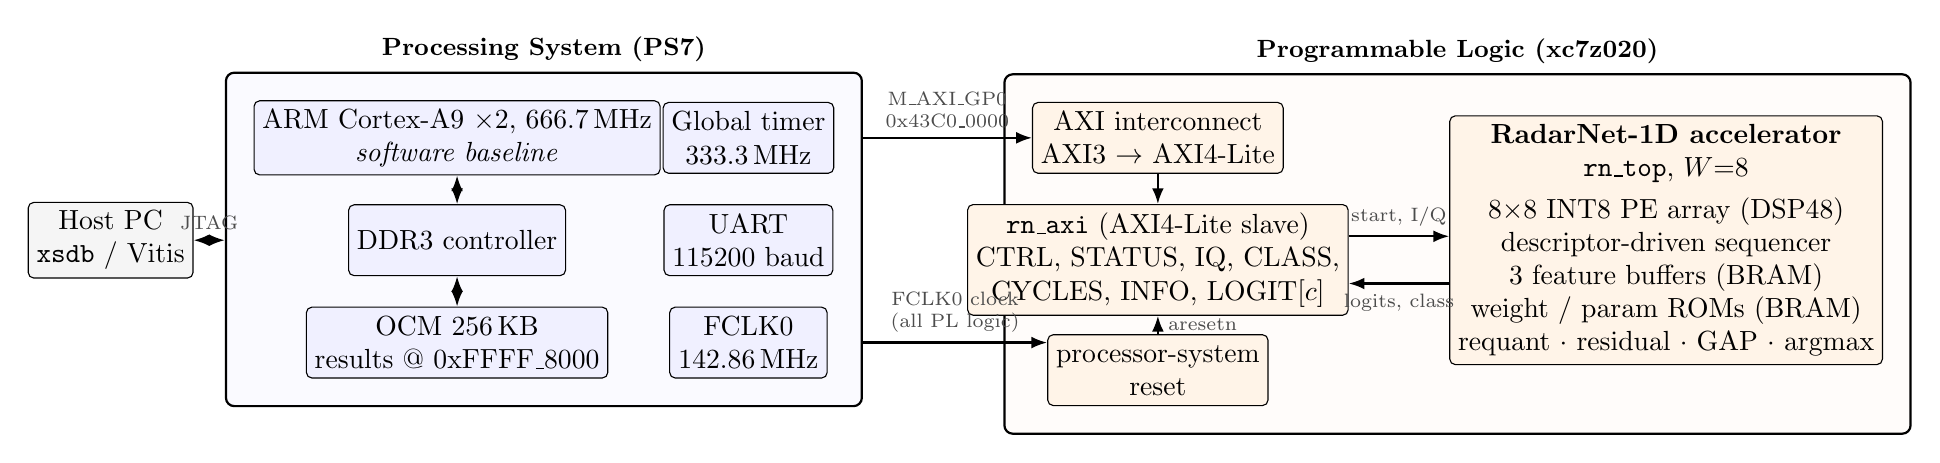
\begin{tikzpicture}[
  blk/.style={draw, rounded corners=2pt, align=center, minimum height=9mm, inner sep=3pt, fill=white},
  ps/.style={blk, fill=blue!6, minimum width=27mm},
  pl/.style={blk, fill=orange!9},
  one/.style={-{Latex[length=2mm]}, thick},
  two/.style={{Latex[length=2mm]}-{Latex[length=2mm]}, thick},
  lbl/.style={font=\scriptsize, text=black!70}]

% ---------------- Processing system ----------------
\node[ps] (cpu) at (0,0)    {ARM Cortex-A9 $\times$2, 666.7\,MHz\\ \textit{software baseline}};
\node[ps] (ddr) at (0,-1.3) {DDR3 controller};
\node[ps] (ocm) at (0,-2.6) {OCM 256\,KB\\ results @ 0xFFFF\_8000};
\node[ps, minimum width=20mm] (gt)   at (3.7,0)    {Global timer\\ 333.3\,MHz};
\node[ps, minimum width=20mm] (uart) at (3.7,-1.3) {UART\\ 115200 baud};
\node[ps, minimum width=20mm] (clk)  at (3.7,-2.6) {FCLK0\\ 142.86\,MHz};
\draw[two] (cpu) -- (ddr);
\draw[two] (ddr) -- (ocm);
\begin{scope}[on background layer]
  \node[draw, thick, rounded corners=3pt, fill=blue!2, inner sep=3.5mm, fit=(cpu)(ocm)(gt)(clk),
        label={[font=\small\bfseries]above:Processing System (PS7)}] (PS) {};
\end{scope}

% ---------------- Programmable logic ----------------
\node[pl, minimum width=26mm] (ic)  at (8.9,0)    {AXI interconnect\\ AXI3 $\rightarrow$ AXI4-Lite};
\node[pl, minimum width=26mm] (axi) at (8.9,-1.55) {\texttt{rn\_axi} (AXI4-Lite slave)\\ CTRL, STATUS, IQ, CLASS,\\ CYCLES, INFO, LOGIT[$c$]};
\node[pl, minimum width=26mm] (rst) at (8.9,-2.95) {processor-system\\ reset};
\node[pl, minimum width=33mm, minimum height=31mm, anchor=west] (acc) at (12.6,-1.3)
  {\textbf{RadarNet-1D accelerator}\\ \texttt{rn\_top}, $W{=}8$\\[3pt]
   $8{\times}8$ INT8 PE array (DSP48)\\ descriptor-driven sequencer\\ 3 feature buffers (BRAM)\\
   weight / param ROMs (BRAM)\\ requant $\cdot$ residual $\cdot$ GAP $\cdot$ argmax};
\draw[one] (ic) -- (axi);
\draw[one] ([yshift=3mm]axi.east) -- node[lbl, above] {start, I/Q} ([yshift=3mm]acc.west |- axi.east);
\draw[one] ([yshift=-3mm]acc.west |- axi.east) -- node[lbl, below] {logits, class} ([yshift=-3mm]axi.east);
\draw[one] (rst) -- node[lbl, right] {aresetn} (axi);
\begin{scope}[on background layer]
  \node[draw, thick, rounded corners=3pt, fill=orange!2, inner sep=3.5mm, fit=(ic)(rst)(acc),
        label={[font=\small\bfseries]above:Programmable Logic (xc7z020)}] (PL) {};
\end{scope}

% ---------------- PS ↔ PL ----------------
\draw[one] (gt.east -| PS.east) -- node[lbl, above, align=center] {M\_AXI\_GP0\\ 0x43C0\_0000} (ic.west);
\draw[one] (clk.east -| PS.east) -- node[lbl, above, align=center] {FCLK0 clock\\ (all PL logic)} (rst.west |- clk.east);

% ---------------- host ----------------
\node[blk, fill=black!4, minimum width=17mm] (host) at (-4.4,-1.3) {Host PC\\ \texttt{xsdb} / Vitis};
\draw[two] (host.east) -- node[lbl, above] {JTAG} (host.east -| PS.west);
\end{tikzpicture}
\end{document}
